\section{Bode-Diagramm von $P_1(s)$}
\begin{figure}[h!]
	\centering
	\includegraphics[scale=1]{../../matlab/exercise/ex_04/ex_04_model.pdf}
	\caption{Simulink-Modell}
\end{figure}

\subsection{Betrachtung der Übertragungsfunktion $P_1(s)$}
Die vorliegende Übertragungsfunktion 
\[
	P_1(s) = \frac{y}{s-x} = \frac{400}{s - (-20.4)} = \frac{400}{s + 20.4}
\]
kann normiert werden, so dass ein typisches PT$_1$-Glied daraus resultiert.
\[
	P_1(s) = \frac{400}{s + 20.4}
		\frac{\left(\frac{400}{20.4}\right)}{1 + \left(\frac{1}{20.4}\right)s}
		\Leftrightarrow \frac{k_p}{1 + T_1 s}
\]
Die Eckwerte eines solchen PT$_1$-Gliedes sind
\begin{itemize}
	\item $|G_0| = 20 \log (kp) = 25.85\mathrm{dB}$
	\item $\omega_0 = \omega(G = G_0 - 3\mathrm{dB}) = \frac{1}{T_1} = 20.4$
	\item $\varphi(\lim_{\omega \rightarrow 0}) = 0^{\circ}$, 
		$\varphi({\omega(G = G_0 - 3\mathrm{dB})}) = -45^{\circ}$,
		$\varphi(\lim_{\omega \rightarrow \infty}) = -90^{\circ}$
	\item $-20\frac{\mathrm{dB}}{\mathrm{Dekade}}$ ab $\omega_0$
\end{itemize}
Das exakte Bodediagramm dieses Übertragungsgliedes ist in der Abbildung
\ref{fig:bode_p1} dargestellt.
\begin{figure}[h!]
	\centering
	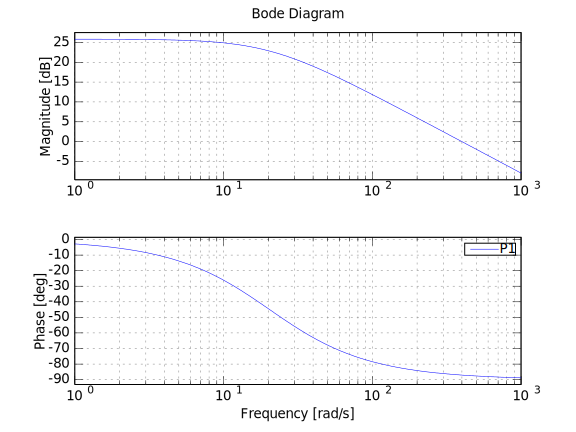
\includegraphics[width=1\textwidth]{../../matlab/exercise/ex_04/bode_p1.pdf}
	\caption{Bode-Diagramm von $P_1(s)$}
	\label{fig:bode_p1}
\end{figure}
